\documentclass[11pt]{report}
\usepackage{amsmath}
\usepackage{mathtools}
\usepackage{amsfonts} 

\title{Sudoku Solver with Simulated Annealing}
\author{Georgios Smyridis}
\date{}

\begin{document}

\maketitle

\section*{Sudoku Puzzle}

Sudoku is a puzzle that is featured in many popular newspapers the past decades and it is a slight modification of Leonard Euler's puzzle, called "Latin Squares". Its objective is straightforward:
\\

\textit{Given an $n^2\times n^2$ square grid divided into $n\times n$ distinct squares, the aim is to fill the each cell so that the following three criteria are met:}
\begin{enumerate}
	\item \textit{Each row of cells contains the integers 1 through $n^2$ exactly once.}
	\item \textit{Each column of cells contains the integers 1 though $n^2$ exactly once.}
	\item \textit{Each $n\times n$ square contains the integers 1 though $n^2$ exactly once.}
\end{enumerate}
\textit{The number n, will be referred as the order of the puzzle in this report.}
\\

One can imagine that it is easy to come up with a valid solution when presented with an empty Sudoku grid. Therefore, in order for the puzzle to be engaging and challenging, it is typical for some of the cels to be pre-filled from the "Sudoku master". The player's aim is then to find a solution, using the fixed pre-filled cells for guidance.

People when they engage in these puzzles, they approach them assuming that there is a unique solution, and they try to come with it using forward chaining logic only. In fact, most define a "good puzzle" as a problem instance that is logic-solvable.

Online one can find all sorts of algorithms that return a solution when provided with a sudoku instance. For many years all of them were, to some degree, dependent on being provided with a problem instance that was designed so that it definitely admits a solution that follows logical steps. However, Sudoku has been proven to be $NP$-complete problem, and thus, there are some initial configurations that cannot be solved in a polynomial time, unless $P=NP$. What this means is that for some sudoku instances, the solution requires also some sort of search.


\section*{Simulated Annealing Approach for Sudoku Puzzles}

In this exercise, we propose a solution to the limitations of logic-based algorithms by applying a method called simulated annealing (SA). The report is structured as follows: First, we provide a general overview of SA as a metaheuristic for approximating global optimization. Then, we demonstrate how SA can be applied to solve puzzles like Sudoku. Afterward, we provide a detailed description of the algorithm we implemented. Finally, we discuss how various control parameters can affect the algorithm's performance and the phenomena that may arise.

\subsection*{What is simulated annealing?}

Simulated annealing is a powerful metaheuristic approach for approximating the global optimum of an optimization problem in a large search space. Essentially, it is a probabilistic method that is useful for finding optimal solutions when traditional exact algorithms, such as gradient descent or branch-and-bound, are computationally expensive or infeasible. By mimicking the physical process of cooling a material, simulated annealing explores the search space and accepts or rejects solutions based on a temperature parameter that decreases over time. This allows for a balance between global exploration and local refinement, enabling the algorithm to find optimal solutions even in complex and high-dimensional search spaces.

\subsection*{Simulated annealing approach for Sudoku}

To adapt the simulated annealing for finding a solution to a Sudoku problem instance, we have to make some definitions. First,
\begin{itemize}
	\item Square will refer to the $n\times n$ area of cells in the grid, separated from each other by bold lines. $\text{square}_{r,c}$ will denote the square that is located in row $i$ and column $j$ in the grid of squares.
	\item The value contained in the cell that is located in the row $r$ and column $c$ of the sudoku grid is going to be denoted $\text{cell}_{i,j}$. If a particular cell is prefilled, then it remains fixed, while otherwise not.
	\item  A complete grid that meets all the Sudoku requirements will be called optimal.
\end{itemize}

\subsubsection{Initialisation and generation of candidate solutions}


To initiate a random candidate solution, we first assign a random value to each non-fixed cell in the Sudoku grid, ensuring that each square contains integers from 1 to $n^2$ exactly once. To generate new candidate solutions, we use the "neighbourhood operator," which selects two different non-fixed cells in the same square and swaps their values. Specifically, we randomly choose a non-fixed cell, denoted as cell$_{i,j}$, and then select another non-fixed cell, cell${k,l}$, in the same square such that cell$_{k,l}\neq$ cell$_{i,j}$. We then swap the values of cell$_{i,j}$ and cell$_{k,l}$.

This approach to generating candidate solutions has the advantage of ensuring that the third requirement of Sudoku, i.e., each square contains integers from 1 to $n^2$ exactly once, is always satisfied. As a result, the total search space for the Sudoku problem is given by the product over all squares of the number of unfixed cells in that square, i.e., $\prod_{r=1}^n\prod_{c=1}^nf(r,c)!$.


\subsubsection{Evaluation of candidate solutions}

Now that we have seen how to generate new candidate solutions, we have to also evaluate them. To accomplish that we have to define a cost function, that is, a function that gives a metric of how far from an optimal solution is the current candidate. The optimal solution will be at a global minimum of the cost function, and thus finding an optimal solution comes down to finding a configuration that minimises the cost function. This is where SA will come into play.

The cost function could have different forms. The cost function we choose to use is calculated in the following way. We are looking at each row $i$, and count the number of integers from $1 $ to $n^2$ that are not present in it. We do the same thing for every column $j$. The total cost function is the total sum. The optimal solution with therefore have vanishing cost.


\subsubsection{Accepting and Rejecting}

Once we have defined a metric to evaluate the quality of a candidate solution, we need a rule to decide whether to accept or reject it. Our acceptance rule is based on the change in the cost function resulting from applying the neighbourhood operator. Specifically, if the cost function is reduced, the candidate solution is accepted. However, we also want to consider candidate solutions that increase the cost function, as it's possible that these may lead to better solutions in the long run.
\\

To achieve this, we introduce a control parameter called the temperature ($T$). If the neighbourhood operator increases the cost function by $\delta$, we accept the candidate solution with a probability of $\exp(-\delta/T)$. This approach allows us to explore the search space more effectively, as we are not limited to only accepting solutions that decrease the cost function.
\\

To optimise our algorithm for speed, instead of calculating the cost function every time and then the difference, we calculate how the swap of two cells affects the cost function. This  shortcut comes immediately from the realisation that swapping two cells affects only two rows and two columns.
\\

It's worth noting that the temperature parameter plays a crucial role in the simulated annealing algorithm. It controls the balance between exploring the search space and exploiting the current solution. At high temperatures, the algorithm is more likely to accept candidate solutions that increase the cost function, allowing for exploration of the search space. As the temperature is lowered, the algorithm becomes more greedy and focuses on exploiting the current solution. The choice of the temperature schedule is therefore an important aspect of the algorithm's performance.


\subsection*{The Simulated Annealing Algorithm}

To solve a given Sudoku problem instance using simulated annealing, we start with an initial candidate solution and explore the search space by repeatedly applying the neighbourhood operator and evaluating the resulting candidate solutions. In our approach, we use the homogeneous SA, which involves a sequence of Markov chains with a specific length, indexed by the temperature.
\\

At each temperature level, we apply the neighbourhood operator a number of times equal to the length of the Markov chains. After generating these new candidate solutions, we evaluate and compare them to the current solution based on the acceptance rule described earlier. We then cool down the temperature based on a predetermined cooling schedule. Specifically, if the cooling rate is $a$, we decrease the temperature as $T_{i+1} = a \cdot T_i$.

We continue this process until an optimal solution is found or we have reached a maximum number of iterations.

\subsubsection{How do we choose the value of the control parameters?}

Choosing the appropriate values for the temperature, cooling rate, and Markov chain length is essential for achieving the desired results in our algorithm. The temperature serves as a control parameter that determines the acceptance rate of candidate solutions generated by the algorithm. If the temperature is set too high, many suboptimal solutions will be accepted, leading to wasted computation time. Conversely, if the temperature is set too low, the algorithm may become too greedy, accepting only marginally better solutions and converging to a local minimum instead of a global one. One approach suggested in [reference] is to set the initial temperature such that it accepts around 80\% of the candidate solutions. This can be achieved by calculating the standard deviation of the cost function for a few applications of the neighbourhood operator and setting it as the initial temperature.
\\

The cooling rate, on the other hand, controls the speed at which the temperature decreases over time. A high cooling rate near 1 will cause slow cooling and result in wasted time and energy. Conversely, a very low cooling rate will cause rapid cooling, potentially leading to premature convergence to suboptimal solutions.
\\

Finally, in [reference], the authors recommend setting the Markov chain length based on the formula:
\begin{align}
ML =\bigg(\sum_{r=1}\sum_{c=1}f(r,c)\bigg)^2
\end{align}
This ensures that the neighbourhood operator will act on all cell pairs statistically. Choosing appropriate values for these parameters can significantly improve the efficiency and effectiveness of the algorithm.


\section*{Performance Analysis}

There are for levels of Sudoku problem instances in our algorithm. The default one is the easiest one, and we'll call it "ulta-easy". The other three are "easy", "medium" and "hard". One can choose the latter with the PreFill(level) method. The conclusions that I drew from trying and testing performance with different parameters are the following:
\begin{enumerate}
	\item The "ultra easy level is pretty much solved within $10^5$ iterations with a really wide range of control parameters.
	\item I have found that choosing the parameters suggested in [reference], does not lead to optimal performance in terms of speed in any case, since, the Markov Chain Length ML is an enormous number. To set these control parameters one should call the method SetIdealControllParameters()
	\item For all levels of Sudoku difficulty, the time and whether it will be solved under the maximum number of iterations heavily depends on the random initial candidate solution.
	\item Statistically however, for the same control parameters, the "easy" sudoku is solved faster than the "medium" one.
	\begin{figure}[ht!]
		\centering
		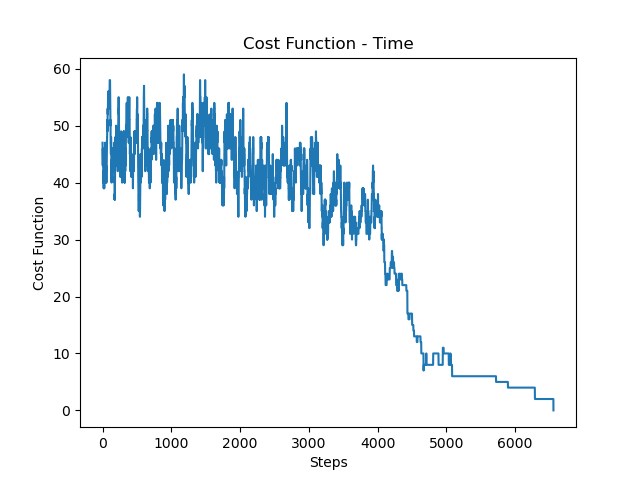
\includegraphics[scale = 0.7]{performance/energies_easy.png}
		\caption{Cost function over time for easy Sudoku problem instance, with control parameters $T=50$, $a=0.9$ and $ML = 10$.}
	\end{figure}
	
		\begin{figure}[ht!]
		\centering
		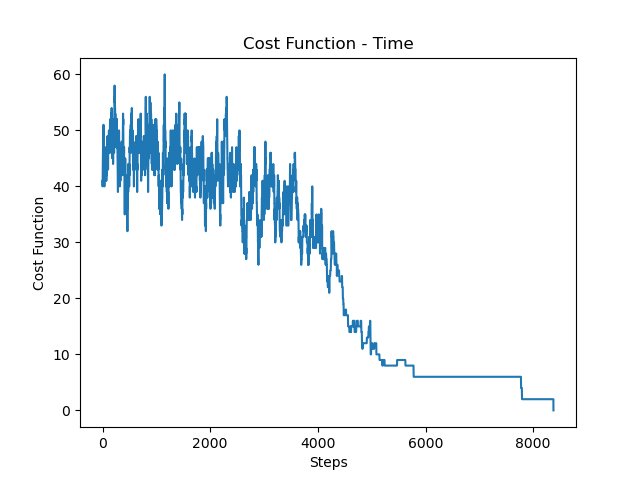
\includegraphics[scale = 0.7]{performance/energies_medium.png}
		\caption{Cost function over time for medium Sudoku problem instance, with control parameters $T=50$, $a=0.9$ and $ML = 10$.}
	\end{figure}
\end{enumerate}


\section*{Improvements}

There are a number of things that I could try to improve the algorithm, as well as test and analyse it better. For potential improvements, I would try to reheat the system, if the cost function does not improve after, say, twenty consecutive iterations. 

 
\section*{Reference}

[reference] DOI 10.1007/s10732-007-9012-8


\end{document}

